\documentclass[a4paper,norsk]{article}
\usepackage{preamble}

\begin{document}
\maketitle
\section*{Exercise 2}
In this exercise we take a look on a deflection of a cable with sine functions. We are presented with the following model for 
a hanging cable of length L with significant tension T and deflection w(x).
\begin{align*}
Tw(x)'' = l(x)
\end{align*}
Assuming constant load $l(x)$, we are presented in the exercise with a scaled model of the vertical deflection $u$ such that
\begin{align*}
u'' = 1 \hspace{5mm}, x\in (0,1) \hspace{5mm} ,u(0)=0 \hspace{2mm} ,u'(1)=0 
\end{align*}

\subsection*{Task a}
To find the exact solution we simply integrate the scaled equation twice with respect to x, giving
\begin{align*}
u(x) = \frac{1}{2}x^2 + Cx + D
\end{align*}
Where $C$ and $D$ are integration constants. Using the boundary conditions we end up with
\begin{align}
u(0) &= D = 0 \hspace{5mm} u'(1) = 1 + C = 0 \hspace{2mm}; C = -1 \\
u(x) &= x(\frac{1}{2}x - 1)
\end{align}

\subsection*{Task b}
Using the suggested function space $\psi_i = sin((2i+1)\frac{x \pi}{2}), \hspace{2mm}i = 0,1...N  $
Defining our element basis function as $\varphi_i$, we must find the unknown coefficients $c_j$ in our expansion
$u = \sum\limits_{j} c_j \varphi_j$ \\ 

\textbf{Galerkin}\\
Using the Galerkin mehtod, let the approximate solution $u(x)$ in some space V such that \\
$V = span {\varphi_0(x), \varphi_1(x),...,\varphi_N(x)}$. In other words we want $u(x)$ to be expressed as a linear combination of our chosen basis functions $\varphi_j$. In the Galerkin method we want the residual R expressed as 
\begin{align*}
R(x;c_0,c_1,...c_N) = u''(x) + f(x) =  \sum\limits_{j} c_j \varphi_j''(x) + f(x)
\end{align*}
to be orthogonal to our space V such that 
\begin{align*}
(R,v) = 0, \hspace{5mm} \forall v \in V
\end{align*}
Where $(R,v)$ denotes the inner product. \newpage

Starting our calculations, the Galerkin method gives us the following equation
\begin{align*}
(u'',v) = (1,v) \hspace{5mm}, (u',v') = -(1,v) \hspace{5mm} ,\forall v \in V
\end{align*}
Here we have used integration by parts, exploiting the boundary condition we end up with the \textit{weak form} of the PDE. Demanding that the residue R is orthogonal to v is equivalent to demanding that R is orthogonal to the basis functions 
$\varphi_i$. By insertion of $R$ and $v$ we get the following equation
\begin{align*}
(\sum\limits_{j}c_j\varphi_j', \varphi_i') = -(1,\varphi_i)
\end{align*}
Which we recognize as a linear system of equations $A_{i,j} c_j = b_j$. Now we start to find the coefficients in matrix 
\textit{A}. 
\begin{align*}
A_{i,j} = \sum\limits_{j} \int_0^1 \varphi_j' \varphi_i' dx
\end{align*}
Since our provided basis is orthogonal, we know that $A_{i,j} = 0$ for i $\neq$ j. Therefore our contributions to the matrix are limited to 

\begin{align*}
A_{i,j} &= \frac{\pi^2}{4}(2i+1)(2j+1) \int_0^1 cos((2i+1)\frac{\pi x}{2}) cos((2j+1)\frac{\pi x}{2}) dx \\
A_{i,j} &= \frac{\pi^2}{4}(2i+1)^2 \int_0^1  cos((2i+1)\frac{\pi x}{2}) dx \\ 
A_{i,j} &= \frac{\pi^2}{4}(2i+1)^2 \frac{1}{2}
\end{align*}
Now we are left with the $b_i$ coefficients, which are calculated straightforward
\begin{align*}
b_i &= -(1,v) = -\int_0^1 \varphi_i dx = -\int_0^1 sin((2i+1)\frac{x\pi}{2}) dx \\
b_i &= - \Big[-\frac{2}{\pi(2i+1)}cos((2i+1)\frac{x\pi}{2})  \Big]_0^1 = -\frac{2}{\pi(2i+1)}
\end{align*}
We know have a complete linear system of equations, and we can find our coefficients simply \newline
\[ c_j = \frac{-\frac{2}{\pi(2i+1)} }{ \frac{\pi^2}{4}(2i+1)^2 \frac{1}{2}} = - \frac{16}{\pi^3(2i+1)^3}  \] \\

\textbf{Least Squares}\\
Using the least squares method our goal is to minimize the square norm of the residual $R$ 
\[ E = (R,R) = \int_\Omega R^2 dx \hspace{3mm} such\hspace{1mm} that \hspace{5mm} 
\frac{\partial E}{\partial c_i} = (R, \frac{\partial R}{\partial c_i} ) = 0\]

First we find the $ \frac{\partial R}{\partial c_i} $ which is used in the calculations
\begin{align*}
\frac{\partial R}{\partial c_i} = \frac{\partial}{\partial c_i} (u'' - 1) = 
\frac{\partial}{\partial c_i}  \sum\limits_{j} c_j \varphi_j'' =
\frac{(2i+1)^2\pi^2}{4} sin((2i+1)\frac{x\pi}{2}) 
\end{align*}
Which we use in our inner product
\begin{align*}
(1 +  \sum\limits_{j} c_j \frac{(2j+1)^2\pi^2}{4} sin((2j+1)\frac{x\pi}{2}),
						  \frac{(2i+1)^2\pi^2}{4} sin((2i+1)\frac{x\pi}{2})) = 0
\end{align*}
Again we see that this inner product is just a linear system of equations. As in Galerkin, we can exploit the orthogonal basis to reduce the sum. 

\begin{align*}
A_{i,j} &= \sum\limits_{j} \int_0^1 \frac{(2j+1)^2\pi^2}{4} sin((2j+1)\frac{x\pi}{2})
						  \frac{(2i+1)^2\pi^2}{4} sin((2i+1)\frac{x\pi}{2})) dx \\
A_{i,j} &= \int_0^1 \frac{(2j+1)^4\pi^4}{16} sin^2((2j+1)\frac{x\pi}{2}) dx 
\end{align*}
Using the trigonometric relation $sin^2(x) = \frac{1}{2} (1 - cos(2x))$ in the integral we end up with the matrix values

\[ A_{i,j} = \frac{1}{2}\frac{\pi^4}{16}(2i+1)^4 \hspace{5mm} ,i = j \]
The $b_i$ values are found by the second integral
\begin{align*}
b_i &= -\int_0^1 \frac{(2i+1)^2\pi^2}{4} sin((2i+1)\frac{x\pi}{2})) dx \\
b_i &= - \frac{(2i+1)^2\pi^2}{4} \Big[-\frac{2}{(2i+1)\pi}cos((2i+1)\frac{\pi x}{2}) \Big]_0^1 =
-\frac{(2i+1)\pi}{2}
\end{align*}
Finally we find our coefficients in the linear system as 
\begin{align*}
c_i = \frac{b_i}{A_{i,j}} = \frac{-\frac{(2i+1)\pi}{2}}{\frac{1}{2}\frac{\pi^4}{16}(2i+1)^4}
= -\frac{16}{\pi^3(2i+1)^3}
Which we observe is the same result as in Galerkin.
\end{align*}
\subsection*{Task c}

\begin{figure}[h!]
  \caption{Numerical solutions against analytical solution}
  \centering
    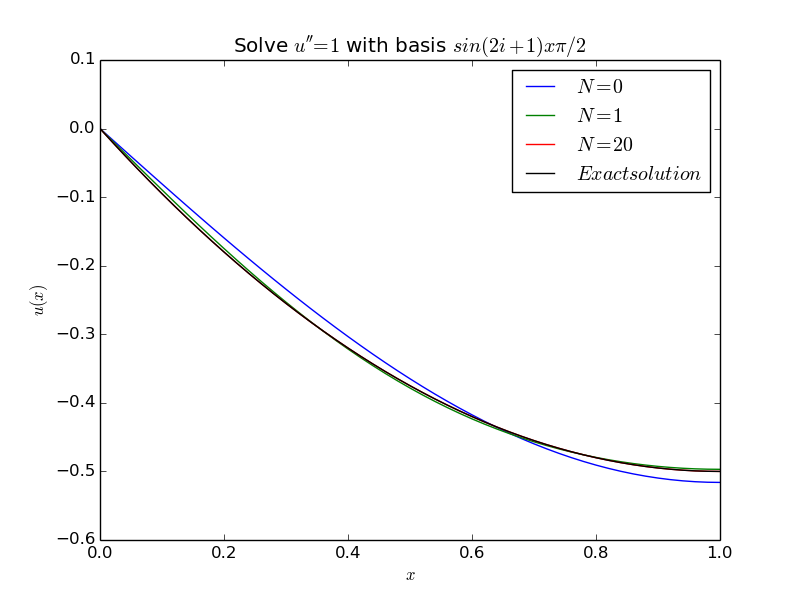
\includegraphics[width=0.8\textwidth]{Taskc.png}
\end{figure}
As we can see we get some decent results from our results in exercise b.

\subsection*{Task d}
This time we are given the basis $\varphi_i = sin((i+1)\frac{x\pi}{2})$. Using the Galerkin method, we observe the integrals from exercise b are more or less similar. Again using the orthogonal property
\begin{align*}
A_{i,j} &= \frac{\pi^2}{4}(i+1)(j+1) \int_0^1 cos((i+1)\frac{\pi x}{2}) cos((j+1)\frac{\pi x}{2}) dx \\
A_{i,j} &= \frac{\pi^2}{8}(i+1)^2 \\
\vspace{5mm}
b_i &=  -\int_0^1 sin((i+1)\frac{x\pi}{2}) dx \\
b_i &= - \Big[-\frac{2}{\pi(i+1)}cos((i+1)\frac{x\pi}{2})  \Big]_0^1 = -\frac{2}{\pi(i+1)}
\end{align*}
Providing the coefficients as 
\begin{align*}
c_i = \frac{b_i}{A_{i,j}} = \frac{-\frac{2}{\pi(i+1)}}{\frac{\pi^2}{8}(i+1)^2} = -\frac{16}{\pi^3(i+1)^3}
\end{align*}
We obsere that the same solution in task \textit{b} appear for \textit{i} chosen as \textit{even}, but we get some additional coefficients \textit{i} chosen as \textit{odd}. Visualisation the solution
\begin{figure}[h!]
  \caption{Numerical solutions against analytical solution}
  \centering
    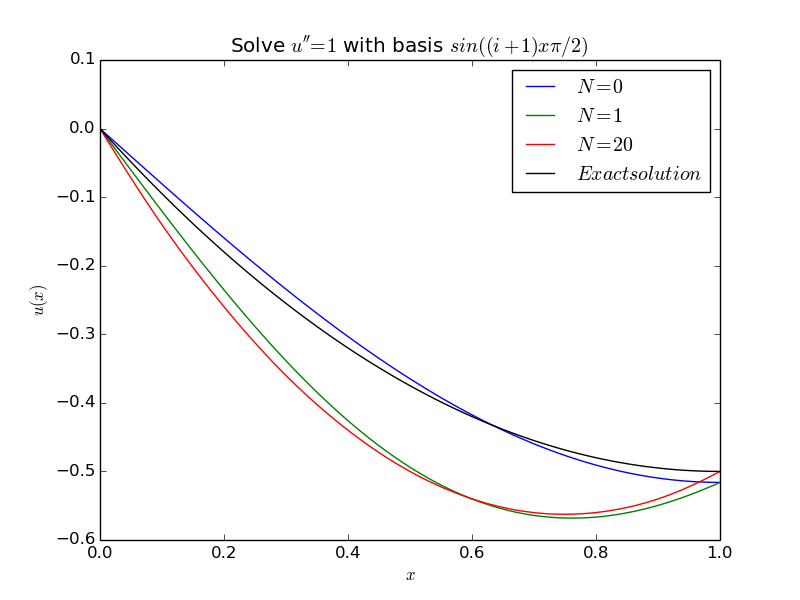
\includegraphics[width=0.8\textwidth]{Taskd.png}
\end{figure}
As we can see the results is a poor representation of the analytical solution. It seems like the additional terms have a bad influence on the numerical solution. 

\subsection*{Task e}
Dropping the symmetry condition at x = 1, we extend the entire scaled cable and we have the following PDE
\begin{align*}
u'' = 1 \hspace{5mm} x \in (0,2) \hspace{5mm}u(0)=u(2)=0 
\end{align*}
Using the basis presented in \textit{d}, $\varphi_i = sin((i+1)\frac{x\pi}{2})$ we use Galerkins method to calculate the slightly new linear system due to the new limits. 
\begin{align*}
A_{i,j} &= \frac{\pi^2}{4}(i+1)(j+1) \int_0^2 cos((i+1)\frac{\pi x}{2}) cos((j+1)\frac{\pi x}{2}) dx \\
\vspace{5mm}
b_i &=  -\int_0^2 sin((i+1)\frac{x\pi}{2}) dx \\
\end{align*}
Again we use orthogonality, leaving us with almost the same integration but with a unexpected new term in $b_i$
\begin{align*}
A_{i,j} &= \frac{\pi^2}{4}(i+1)^2\\
b_i &= \frac{2}{\pi(i+1)}cos((i+1)\pi)-1 )
\end{align*}
Taking a closer look at $b_i$ we observe that we only get contribution for \textit{i} chosen as even, as \textit{i} chosen a odd results in zero in the bracket. Thus the computed coefficients $c_j$ alternates as follows

\[
  c_j = \frac{b_j}{A_{i,j}} = \left\{\def\arraystretch{1.2}%
  \begin{array}{@{}c@{\quad}l@{}}
    0 & \text{if i is \textit{odd}}\\
    -\frac{16}{(i+1)^3\pi^3} & \text{if i is \textit{even}}\\
  \end{array}\right.
\]
The numerical solution yields
\begin{figure}[h!]
  \caption{Numerical solutions against analytical solution}
  \centering
    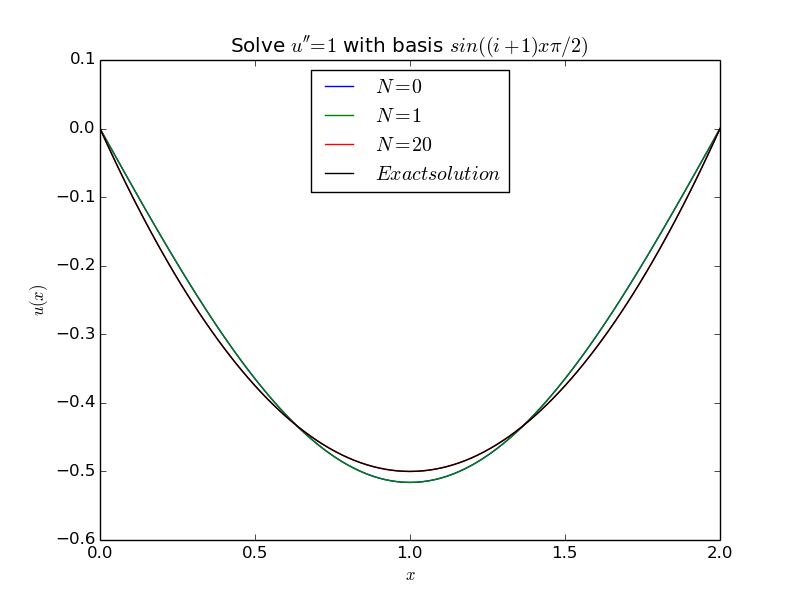
\includegraphics[width=0.8\textwidth]{Taske.png}
\end{figure}
The reason this basis worked for the expanded scaled PDE, rather than the symmetry condition in exercise \textit{d} comes from the fact that the extra coefficients appearing from i chosen as \textit{odd}. When we chose \textit{odd} values, we insert basisfunctions which are anti-symmetric at x=1. When we chose $i =3,7,11,15..$ we are fine due to the fact that these basis functions have integer-periods in the interval [0,1], which will yeild a integral = 0. While the other contribution from  $i =5,9,13,17..$ have non-integer period and also non-symmetric, the derivative is nonzero where we demand as a condition u(1)' = 0.


\newpage
\section*{Exercise 5}
In this exercise we are studying the same problem as in exercise 2, but this time we are to solve the equation using two linear P1 elements. Firstly our domain is again $x \in (0,1),$ leaving us with two elements. Let $\Omega^{(e)}$ denote a chosen element, giving us the following:
\begin{align*}
u'' = 1 \hspace{5mm} u(0)=0, u'(1)=0 \hspace{5mm} \Omega^{(0)} = [0, 0.5] \hspace{2mm} \Omega^{(1)} = [0.5,1]
\end{align*}
Now as in exercise 2, by using Galerkins method and applying integration by parts we get
\begin{align*}
(u',v') = -(1,v) \hspace{2mm}\forall v \in V
\end{align*}
Further on we are tasked to check out to methods of incorporating $u(0)=0$.

\subsection{Method 1}
 As in exercise 2 we want to represent the approximation of u as $u = \sum\limits_{j} c_j \varphi_j$, but this time we want to check how exluding the unknown at x = 0 effects the solution. In other words $u= c_0\varphi_1 + c_1\varphi_2 $. \\
 This time our basis functions $\varphi_i$ are chosen as hatfunctions in evenly distributed elements such that
\[
  \varphi_i = \left\{\def\arraystretch{1.2}%
  \begin{array}{@{}c@{\quad}l@{}}
    x < x_{i-1}  & 0\\
    x_{i-1} < x < x_{i} & \frac{x-x_{i-1}}{x_i-x_{i-1}}\\
    x_{i} < x < x_{i+1} & 1-\frac{x-x_i}{x_{i+1}-x_i} \\
    x \geq x_{i-1} &0
  \end{array}\right.
\]
for each $x_i$ and corresponding $\varphi_i$ in the elements. Moving on to the calculations we will use Galerkin to compute the approximation. 
For the Galerkin method we recognize 
\begin{align*}
A_{i,j} = (\varphi_i,\varphi_j)
b_i = (1,\varphi_i)
\end{align*}

Remembering that the calculations are a linear system we let matrix $A_{i}{j}$ be a sum of contributions from each element in $\Omega$ such that \[A_{i}{j}= \sum\limits_{e} A_{i,j}^{(e)}\] where $e$ represents a given element. 
Since we are exluding the unknown at x = 0, we only get one contribution into the global coefficient matrix and $b_i$ matrix.
\begin{align*}
A_{1,1}^{(0)} &= \int_\Omega \varphi_1' \varphi_1' dx = \int_0^{\frac{1}{2}} \Big[\frac{\partial}{\partial x} 
\frac{x-x_0}{x_1-x_0}\Big]_0^{\frac{1}{2}} dx = \Big[\frac{x}{h^2}\Big]_0^{\frac{1}{2}} = \frac{1}{h}(1) \\ 
b_1 &= -\int_\Omega \varphi_1 dx = -\int_0^{\frac{1}{2}} \frac{x-x_0}{x_1-x_0} dx = -\frac{h}{2}(1)
\end{align*}
Since we are operation with a even distanced mesh, every distance between mesh points is such that
$x_i-x_{i-1} = h = \frac{1}{2}$
Now for element number 2 we have
\begin{align*}
A_{0,1}^{(1)} &= \int_\Omega \varphi_0' \varphi_1' dx = \int_{\frac{1}{2}}^1 \Big[\frac{\partial}{\partial x} 
(1-\frac{x-x_1}{x_{i+1}-x_i})'(\frac{x-x_1}{x_2-x_1})' dx =
 \Big[-\frac{x}{h^2}\Big]_{\frac{1}{2}}^1 = -\frac{1}{h}\\
b_2 &= -\int_\Omega \varphi_2 dx = -\int_{\frac{1}{2}}^{1} \frac{x-x_0}{x_1-x_0} dx = -\frac{h}{2}(1)
\end{align*}
It can be shown that $A_{i,i-1} = A_{i,i+1}$. Using this fact and symmetry we get the global coefficient matrix as

\[ \frac{1}{h}
\begin{bmatrix}
2 & -1 \\ -1 & 1
\end{bmatrix}
\begin{bmatrix}
c_0\\ c_1
\end{bmatrix}
= -\frac{h}{2}
\begin{bmatrix}
2\\1 
\end{bmatrix}
\]
Using numpy gives the output
\begin{align}
c_0 = -\frac{3}{8} \hspace{5mm} c_1 = \frac{1}{2}
\end{align}
Which results in the numeric value $\frac{1}{2}\hspace{3mm} \frac{3}{8}$, which is the analytical solution at each point.

\subsection*{Method 2}
In this subtask we are to keep the unknown at x=0, and modify the linear system of equations. Now we want our approximation as $u = c_0 \varphi_0 + c_1 \varphi_1 + c_2 \varphi_2$ Using  $A_{i,i-1} = A_{i,i+1}$ and symmetry of elements due to even spaced mesh $x_i-x_{i-1} = h$ and reusing calculations from method 1, our global coefficient matrix yields 
\[ \frac{1}{h}
\begin{bmatrix}
1 & -1 & 0 \\
-1 & 2 & -1 \\
0 & -1 & 1
\end{bmatrix}
\begin{bmatrix}
c_0\\ c_1 \\ c_2
\end{bmatrix}
= -\frac{h}{2}
\begin{bmatrix}
1 \\ 2 \\ 1 
\end{bmatrix}
\]
Now we have to modify the linear system to maintain Dirichlet condition at $x=0$. We have to demand $c_0 = 0$. Some manipulation of the matrix results in a remaining 2x2 matrix, which is the same system as we reached in method 1, which yields the same solution for $c_0 = 0$


\end{document}


